\chapter{\bfseries Materiais e Métodos}


O sistema foi desenvolvido na forma de aplicação \textit{web}. Para isso, foram utilizadas os materiais descritos na Tabela \ref{tabela: materiais}.

\begin{center}
\begin{longtable}{|C{3.0 cm}|c|C{4.5 cm}|L{5cm}|}
\caption{Materiais utilizados no desenvolvimento do sistema}
\label{tabela: materiais} \\

\hline \multicolumn{1}{|c|}{\textbf{Material}} & \multicolumn{1}{c|}{\textbf{Versão}} & 
\multicolumn{1}{c|}{\textbf{Disponível em}} &  
\multicolumn{1}{c|}{\textbf{Aplicação}}  \\\hline

\endfirsthead

\multicolumn{4}{l}%
{{\bfseries \tablename\ \thetable{} -- na página anterior}} \\
\hline \multicolumn{1}{|c|}{\textbf{Material}} &
\multicolumn{1}{c|}{\textbf{Versão}} &
\multicolumn{1}{c|}{\textbf{Disponível em}} &
\multicolumn{1}{c|}{\textbf{Aplicação}}  \\ \hline 
\endhead

\hline \multicolumn{4}{|r|}{{Continua na página seguinte}} \\ \hline
\endfoot

\hline \hline
\endlastfoot

Apache TomCat & 8.5 & http://\-tomcat.\-apache.\-org/ & Container de Servlets 
que implementa as tecnologias Java, funciona como um servidor para aplicações em Java. \\ \hline
Axure RP & 8.1 & https://www.axure.com/ & Ferramenta rápida de criação de diagramas, wireframes, protótipos e especificações para websites. \\ \hline
Bootstrap                        & 3.3.6           & http://getbootstrap.com/                                           & Framework de estilizações de páginas por meio de Cascading Style Sheets (CSS).                                                                         \\ \hline
CSS                              & 3               & https://www.w3.org/css/                                            & Linguagem que serve para “descrever” a aparência/estilo de uma página web por meio de folhas de estilo em cascata.                                     \\ \hline
Hibernate                        & 5.1.0           & http://hibernate .org/                                             & Para mapeamento objeto relacional e persistência de dados.                                                                                             \\ \hline
HTML                             & 5.0             & https://www.w3.org/
html/                                           & Linguagem de marcação de textos utilizada para desenvolvimento de interfaces de aplicações.                                                            \\ \hline
Java EE                          & 8.0             & http://www.oracle.com/
technetwork/java/javaee/
downloads/index.html & Linguagem para desenvolvimento da aplicação.                                                                                                           \\ \hline
JQuery                           & 2.2.4           & https://jquery.com/                                                & Biblioteca JavaScript utilizada no desenvolvimento da interface.                                                                                       \\ \hline
Maven                            & 4.0             & https://\-maven.\-apache.\-org/                                          & Modelagem do projeto e gerenciamento de dependências.                                                                                                  \\ \hline
MySQL Server                     & 5.7             & https://dev.mysql.com/
downloads/mysql/                             & Sistema de gerenciamento de banco de dados (SGBD), que utiliza a linguagem Structured Query Language (SQL).                                            \\ \hline
MySQL Workbench                  & 6.3             & https://dev.mysql.com/
downloads/mysql/                             & Modelagem do Banco de Dados do Sistema.                                                                                                                \\ \hline
NetBeans                         & 8.1             & https://netbeans.org/                                              & Integrated Development Environment (IDE) para desenvolvimento da aplicação.                                                                            \\ \hline
VRaptor IV                       & 4.2.0           & http://www.vraptor.org/                                            & Framework para desenvolvimento ágil de sistemas web com a linguagem de programação Java. \\ \hline
\end{longtable}
\end{center}

As ferramentas descritas na Tabela \ref{tabela: materiais} foram utilizadas em algum ou ambos ciclos de desenvolvimento. 


Após a configuração do Hibernate foram criadas as classes de modelo conforme o diagrama de entidade-relacionamento, apresentado , juntamente com as anotações necessárias utilizadas pelo Hibernate para realizar o mapeamento das classes, como apresentado no .

\begin{codigo}
\caption{Caption2 do quadro}
\label{codigo_modelo2}

\begin{lstlisting}[language=Java]
@Entity
public class Questao implements Serializable {
    @Id
    @GeneratedValue(strategy = GenerationType.IDENTITY)
    private Integer id;
    
    @Column(length = 5000)
    private String enunciado;
    
    @Column(length = 3000)
    private String alternativaA;
    
    @Column(length = 3000)
    private String alternativaB;
    
    @Column(length = 3000)
    private String alternativaC;
    
    @Column(length = 3000)
    private String alternativaD;
    
    private Integer alternativaCorreta;
	... 
}
\end{lstlisting}
\end{codigo}

O  apresenta uma parte da classe LoginController.java. O uso dos padrões do \textit{framework} pode ser visto nas anotações acima dos métodos públicos, que indicam o método de requisição conforme a semântica dos métodos do \textit{HyperText Transfer Protocol} (HTTP) (Get, Post, Put, \textit{Patch}, \textit{Delete}, \textit{Head}, \textit{Options}, \textit{Connect} e \textit{Trace}), requisições enviadas que não sejam do mesmo tipo anotado no método são rejeitadas automaticamente.






No texto, use assim:

% Também é possível especificar outra ordem de posicionamento como [htb]:

% \begin{quadro}%[htb]
% \caption{\label{quadro_modelo}Caption do quadro}
% Este é o conteúdo do quadro.
% \end{quadro}



% %inicio_quadro com longtable
% \renewcommand\LTcaptype{quadro} % Especifica para utilizar o contador e nome do ambiente `quadro`
% \begin{longtable}[]{@{}cl@{}}
% \caption{Título do quadro\label{quadro_model1o}}
% \endfirsthead

% \caption*{Fonte: Autor.} \\
% \endfoot

% % a tabela aqui
% \begin{tabular}{cc}
% 123 & 456\\
% 123 & 456\\
% \end{tabular}

% \end{longtable}
% \renewcommand\LTcaptype{table} % Restaura para próximas tabelas utilizar o ambiente `table`
% %fim_quadro com longtable


\begin{figure}
	\caption{A boat.}
	
\includegraphics[width=\linewidth]{2-textuais/figs/Overleaf-750x300.jpg}
	\label{fig:boat1}
	\legend{Fonte: Autor.}
\end{figure}

Figure \ref{fig:boat1} shows a boat.


\begin{mapa}
	\caption{A boat.}
	
\includegraphics[width=\linewidth]{2-textuais/figs/Overleaf-750x300.jpg}
	\label{map:boat2}
	\legend{Fonte: Autor.}
\end{mapa}

Figure \ref{map:boat2} shows a boat.

\begin{desenho}
	\caption{A boat.}
	
\includegraphics[width=\linewidth]{2-textuais/figs/Overleaf-750x300.jpg}
	\label{des:boat3}
	\legend{Fonte: Autor.}
\end{desenho}

Figure \ref{des:boat3} shows a boat.

\begin{figure}[ht!]
	\centering
	\caption{The same cup of coffee. Two times.}
	\begin{subfigure}[b]{0.4\linewidth}
		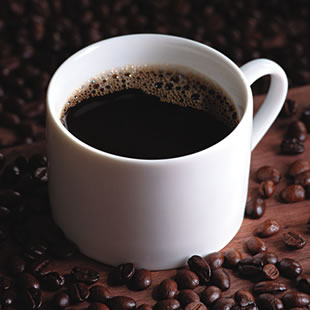
\includegraphics[width=\linewidth]{2-textuais/figs/coffee.jpg}
		\caption{Coffee.}
	\end{subfigure}
	\begin{subfigure}[b]{0.4\linewidth}
		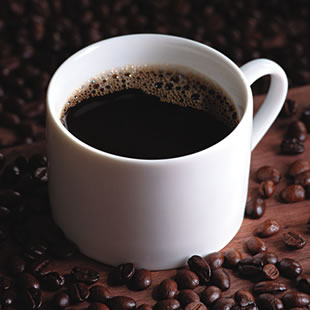
\includegraphics[width=\linewidth]{2-textuais/figs/coffee.jpg}
		\caption{More coffee.}
	\end{subfigure}
	\label{fig:coffee1}
	\legend{Fonte: Autor.}
\end{figure}


\begin{figure}[ht!]
	\centering
	\caption{The same cup of coffee. Two times.}
	\begin{subfigure}[b]{0.4\linewidth}
		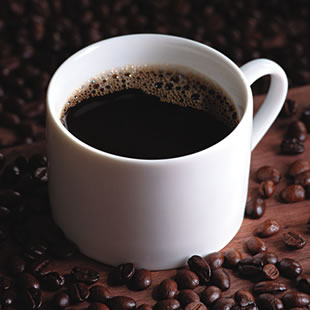
\includegraphics[width=\linewidth]{2-textuais/figs/coffee.jpg}
		\caption{Coffee.}
	\end{subfigure}
	\begin{subfigure}[b]{0.4\linewidth}
		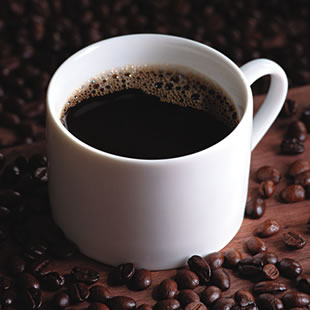
\includegraphics[width=\linewidth]{2-textuais/figs/coffee.jpg}
		\caption{More coffee.}
	\end{subfigure}
	\label{fig:coffee22}
	\legend{Fonte: Autor.}
\end{figure}
    
\begin{figure}[ht!]
	\centering
	\caption{The same cup of coffee. Again.}
	\begin{subfigure}[b]{0.2\linewidth}
		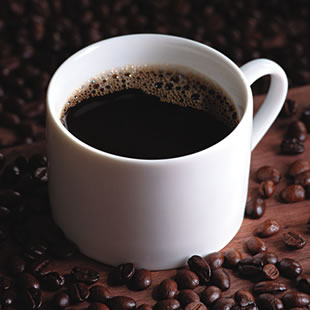
\includegraphics[width=\linewidth]{2-textuais/figs/coffee.jpg}
		\caption{Tasty coffee.}
	\end{subfigure}
    \begin{subfigure}[b]{0.6\linewidth}
		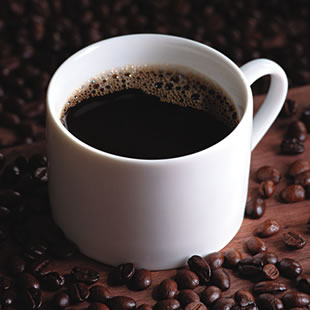
\includegraphics[width=\linewidth]{2-textuais/figs/coffee.jpg}
		\caption{Too much coffee.}
	\end{subfigure}
	\label{fig:coffee2}
	\legend{Fonte: Autor.}
\end{figure}

\begin{figure}[ht!]
	\centering
	\caption{The same cup of coffee. Multiple times.}
	\begin{subfigure}[b]{0.2\linewidth}
		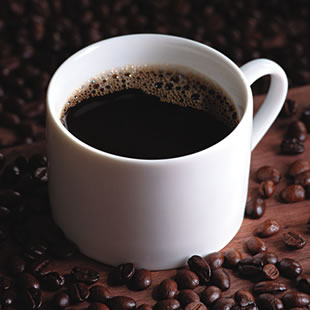
\includegraphics[width=\linewidth]{2-textuais/figs/coffee.jpg}
		\caption{Coffee.}
	\end{subfigure}
	\begin{subfigure}[b]{0.2\linewidth}
		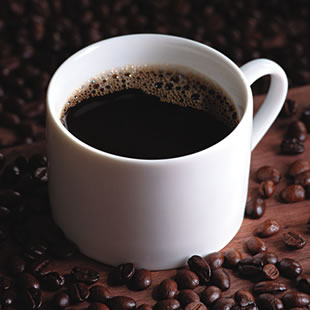
\includegraphics[width=\linewidth]{2-textuais/figs/coffee.jpg}
		\caption{More coffee.}
	\end{subfigure}
	\begin{subfigure}[b]{0.2\linewidth}
		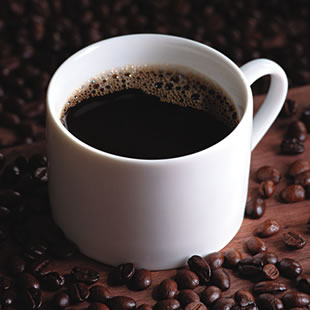
\includegraphics[width=\linewidth]{2-textuais/figs/coffee.jpg}
		\caption{Tasty coffee.}
	\end{subfigure}
    \begin{subfigure}[b]{0.5\linewidth}
		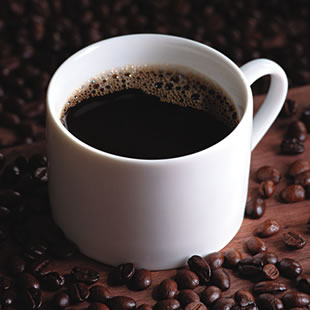
\includegraphics[width=\linewidth]{2-textuais/figs/coffee.jpg}
		\caption{Too much coffee.}
	\end{subfigure}
	\label{fig:coffee3}
	\legend{Fonte: Autor.}
\end{figure}